\subsection{Fase di analisi}

\subsubsection{Prospetto orario}
La seguente tabella rappresenta la distribuzione oraria per ogni componente del gruppo nella fase di analisi:
\begin{table}[H]
\begin{center}
\rowcolors{2}{gray!25}{white}
\renewcommand{\arraystretch}{1.25}
\begin{tabular}{ m{0.20\textwidth}<{\centering}  m{0.06\textwidth}<{\centering} m{0.06\textwidth}<{\centering} m{0.06\textwidth}<{\centering}  m{0.06\textwidth}<{\centering}  m{0.06\textwidth}<{\centering}  m{0.06\textwidth}<{\centering}  m{0.20\textwidth}<{\centering}   }
	\rowcolor{darkblue}
	\textcolor{white}{\textbf{Componente}} &\textcolor{white}{\textbf{Re}}&\textcolor{white}{\textbf{Pt}}&\textcolor{white}{\textbf{An}}&\textcolor{white}{\textbf{Am}}&\textcolor{white}{\textbf{Pr}}&\textcolor{white}{\textbf{Ve}}&\textcolor{white}{\textbf{Ore complessive}}\\ 
	Edoardo Pavan & 2 & 0 & 5 & 5 & 0 & 4 & 16 \\	
	
	Francesco Protopapa & 4 & 0 & 16 & 0 & 0 & 7 & 27 \\

	Greta Cavedon & 6 & 0 & 16 & 0 & 0 & 6 & 28 \\
	
	Luciano Wu & 0 & 0 & 16 & 0 & 0 & 3 & 19 \\
	
	Matteo Basso & 3 & 0 & 5 & 5 & 0 & 7 & 20 \\
	
	Michele Gatto &  0 & 0 & 5 & 9 & 0 & 2 & 16 \\
	
	Pietro Villatora & 0 & 0 & 4 & 8 & 0 & 9 & 21 \\
	
	\textbf{Ore totali ruolo} & 15 & 0 & 67 & 27 & 0 & 38 & 147\\

\end{tabular}
\caption{Distribuzione oraria per ogni componente nella fase di analisi}
\end{center}
\end{table}

La tabella può essere rappresentata anche in forma visiva dal seguente istogramma: 
\begin{figure}[H]
\centering
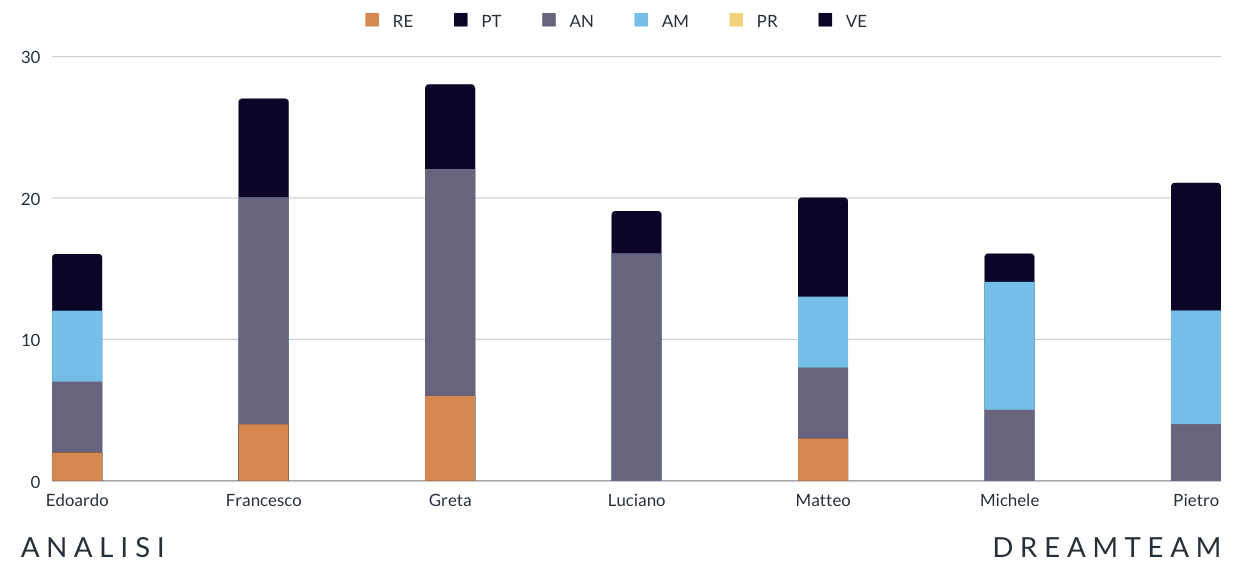
\includegraphics[scale=0.65]{Sezioni/SezioniPreventivo/grafici/Analisi.png}
\caption{Istogramma della ripartizione delle ore durante il periodo di analisi}
\end{figure}

\subsubsection{Prospetto economico}
La seguente tabella rappresenta le ore totali dedicate ad ogni ruolo e il costo in euro:

\begin{table}[H]
\begin{center}
\rowcolors{2}{gray!25}{white}
\renewcommand{\arraystretch}{1.5}
\begin{tabular}{ m{0.3\textwidth}<{\centering}  m{0.2\textwidth}<{\centering} m{0.2\textwidth}<{\centering}}
	\rowcolor{darkblue}
	\textcolor{white}{\textbf{Ruolo}}&\textcolor{white}{\textbf{Totale ore}}&\textcolor{white}{\textbf{Costo totale (\euro)}}\\ 

	Responsabile  & 15 &  450\\	
	
	Progettista & 0 &  0 \\
	
	Analista & 67 &  1675\\

	Amministratore & 27 &  540\\
	
	Programmatore & 0 &  0\\
	
	Verificatore & 38 &  570\\
	
	\textbf{Totale} & 147 &  3235 \\
	
\end{tabular}
\caption{Prospetto del costo per ruoli nella fase di analisi}
\end{center}
\end{table}

La tabella può essere rappresentata anche in forma visiva dal seguente aerogramma:
\begin{figure}[H]
\centering
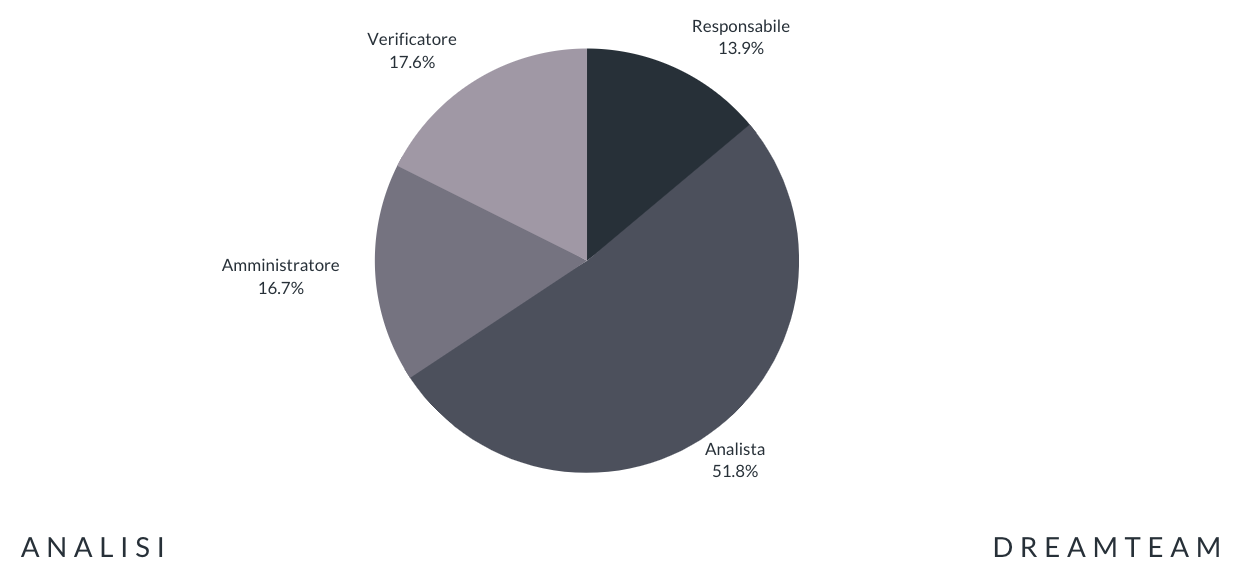
\includegraphics[scale=0.65]{Sezioni/SezioniPreventivo/grafici/Analisi_costi.png}
\caption{Grafico a torta della ripartizione per ruolo dei costi nella fase di Analisi}
\end{figure}



